\chapter{Materials and methods}
\label{Chap3}
Description expériences et machines
\section{Powder follow-up}

\subsection{Sieving}

\subsection{Grain size and distribution}

\subsection{Composition}

%\subsection{Drying}

\section{Fabrication process parameters}
The same direct metal printer (DMP) was used to fabricate all specimens throughout this work. It is a \textit{ProX DMP 200} printer, manufactured by \textit{3D Systems} (see figure \ref{fig:Printer}). It uses a laser with a theoretical maximal power of 300 [W] and wavelength $\lambda$ = 1070 [nm] \parencite{3D}. Its actual maximal power is $P_{max}=273.6 [W]$. [QUEL EST LE SPOT SIZE?]  The maximal envelope capacity of the machine (W x D x H) is 140 x 140 x 125 [mm]. Its typical accuracy is +/- 50 [$\mu m$] for small parts and +/- 0.2\% for large parts. It allows for the set-up of a protection atmosphere. However, it does not integrate any heating feature for the build bed.\\

\begin{figure}[th]
\centering
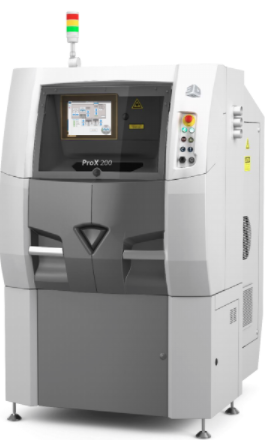
\includegraphics[scale=0.7]{Images/Printer}
\decoRule
\caption[ProX DMP 200 printer]{ProX DMP 200 printer (from the user's ProX DMP 200 general instructions document).}
\label{fig:Printer}
\end{figure}

In this thesis, argon was used as shielding gas. The composition of the gas environment was monitored so as to keep $p_{O2}$ < 500 [ppm]. Laser compensations were set to take into account the excess energy at the start and end of the scanning vectors (see figure \ref{fig:Compens}). These were chosen in accordance with the manufacturer recommendations (figure \ref{fig:Compens1}). Values for h and t were respectively set to 100 [$\mu m$] and 30 [$\mu m$]. The other process parameters were varied so as to optimize the properties of the built specimens. Educated guesses were made based on literature and previous works done at the UCL. The parameters used are resumed in annex \ref{ppa}. Batches were named in the format X200-\textit{yymmdd}. The prefix "X200" refers to the DMP used. It is followed by the date of printing (6 digits). Recycled powder was used for every batch except for X200-180222 and X200-180228. In the case of samples with contour scanning strategy, the contours were pre scanned for each powder layer with the same P and $v_s$ used for the bulk. \\

\begin{figure}[th]
\centering
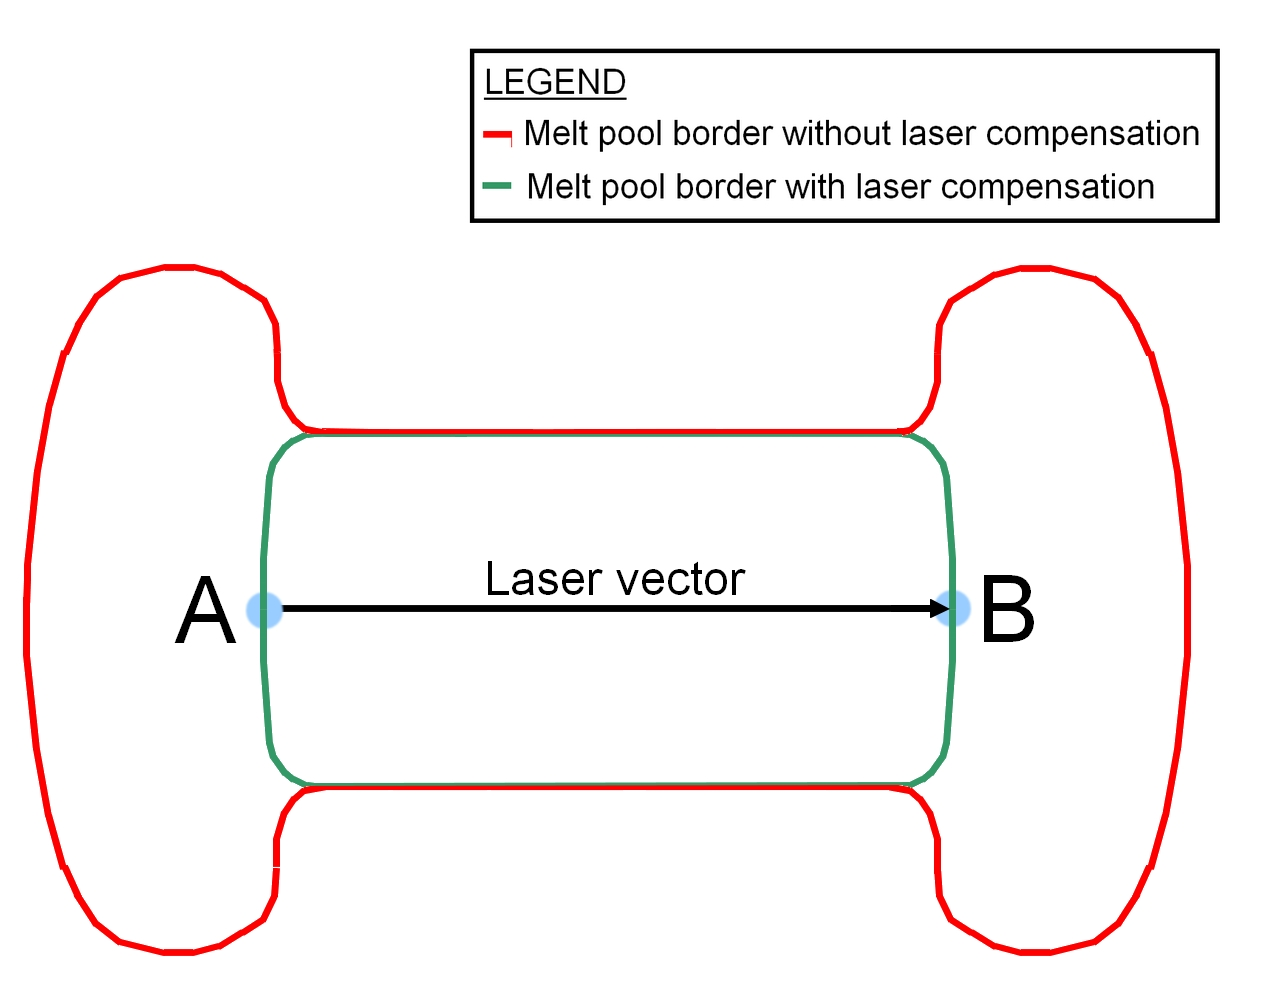
\includegraphics[scale=0.3]{Images/Compens}
\decoRule
\caption[Melt pool contours with and without laser compensation (exaggeration)]{Melt pool contours with and without laser compensation (exaggeration).}
\label{fig:Compens}
\end{figure}

\begin{figure}[th]
\centering
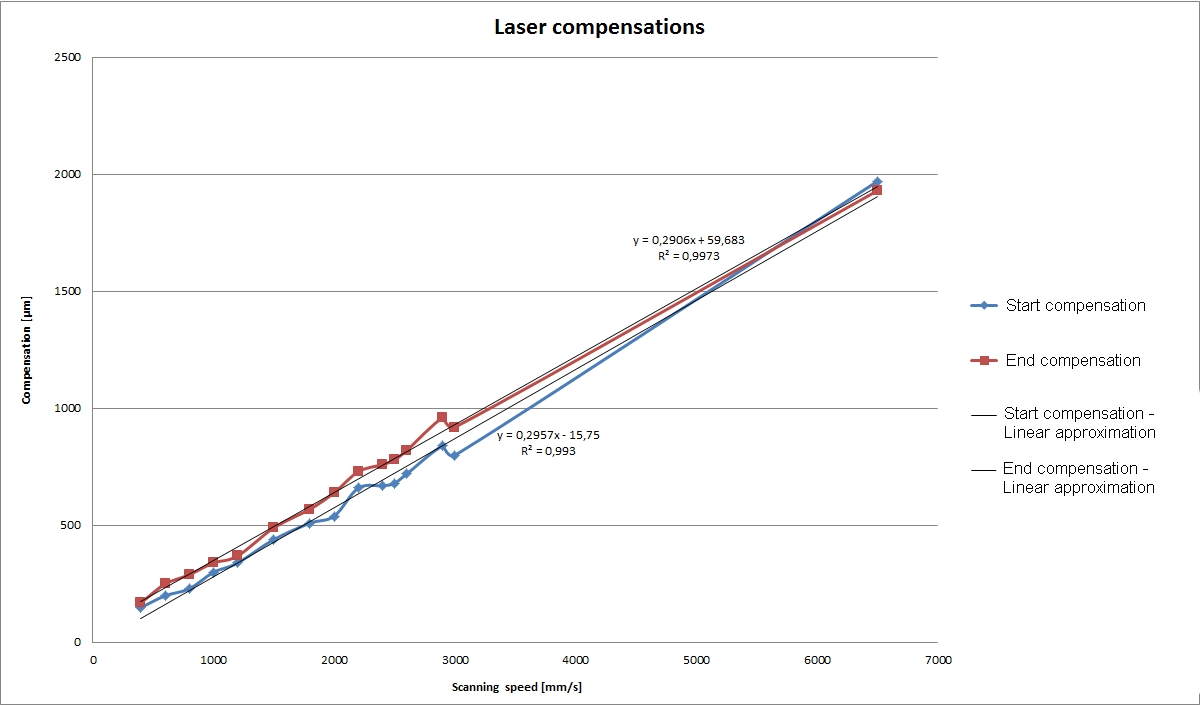
\includegraphics[scale=0.45]{Images/Compens1}
\decoRule
\caption[Laser compensations as a function of the scanning speed (as recommended by the manufacturer)]{Laser compensations as a function of the scanning speed (as recommended by the manufacturer).}
\label{fig:Compens1}
\end{figure}

All batches were first prepared on \textit{DMP ProX Manufacturing}, a dedicated CAD software. It enabled to chose the values for the parameters previously mentioned, as well as the position of the specimens. The scanning order was automatically chosen. Figures with detailed specimens positions, denominations, scanning orders and sintering durations are available in annex \ref{mda}.\\

An island scanning strategy was chosen on account of research done on the subject (see section \ref{pp}). It is a hexagonal pattern with ???  [OVERLAP? TAILLE DES HEXAGONES?]\\

Insérer images de trajets du laser.\\

[Parler des éprouvettes utilisées]\\

\section{Heat treatments}

The heat treatments were conducted inside a unique oven of the ... model, manufactured by ..., which is able to reach a temperature of 400$^\circ$ C. Samples temperature data was obtained through a thermocouple welded to the sample surface. [Méthode de soudage, élévation de la température durant l'opération] The data was displayed and saved every 10 seconds, with a precision of 0.1$^\circ$ C, thanks to a ..., connected to the thermocouple (see Fig. for both devices). \\

Samples that were subject to a heat treatment were named in a particular format, to ease distinction between them. They received the name of the batch, followed by "TT-\textit{holdingtemperature-holdingtime-specific conditions}".

\section{Characterisation}

\subsection{Density}

\subsubsection{Hydrostatic weighing}

Multiple methods were considered to estimate the relative density of the fabricated specimens. The first one is hydrostatic weighting (also called hydrodensitometry). It is a direct application of the well-known Archimedes' principle, which can be stated as follows: " When a body is (partially or totally) immersed in a fluid, the upthrust on the body is equal to the weight of fluid displaced." \parencite{ADictionaryofPhysics}. By weighing each pieces in air and in water - giving respectively values of dry weight $W_a$ and underwater weight $W_w$ - one can calculate the apparent density $\rho_a$ \parencite{MethArch}:

$$\rho_a=\frac{W_a}{W_a-W_w} \cdot \rho_w $$

where $\rho_w$ is the water density. The apparent relative density $\rho_{a,rel}$ of the specimens can then be calculated with:

$$\rho_{a,rel} = \frac{\rho_a}{\rho_b} $$

where $\rho_b = 2.68 [\frac{g}{mm^3}]$ is the theoretical bulk density of AlSi10Mg \parencite{Bulk}. All weightings were done with a \textit{Sartorius BP121S} analytical balance with precision of 0.1 [mg] \parencite{Balance}. Samples were immersed in demineralised water for more than twelve hours before the measurements to impregnate them. The weightings were also done in demineralised water. Water temperature was measured with a precision glass thermometer to compute $\rho_w$ as accurately as possible thanks to tabulated values \parencite{Eau}. Multiple measurements were done for each sample in order to increase the method's reliability. \\

The technique was employed with "as-built" and polished cubes. This second option reduces the risks of air trapping by the surface roughness, which can distort the results (by overestimating the closed porosities volume). \textcolor{red}{A mettre dans la discussion en fait peut-être?} %to observe potential inhomogeneous distributions of the closed porosities in the specimens.
All six faces of the tested cubes were polished with P320 silicon carbide sandpaper sheets and briefly with P1200 ones.\\

\subsubsection{Relative optical density image analysis}

Another method was used to estimate the relative density of the various samples: the relative optical density image analysis (RODIA). For this purpose, the samples were cut with a micro-cutting machine and underwent the polishing routine detailed in table \ref{tab:pol}. Pictures of the polished sections were then taken under the optical microscope.[Infos sur le microscope, grossissement] The pictures were taken with a \textit{Huawei Mate 10 Lite} smart-phone trough the lens of the microscope. The used camera has a resolution of 16 [MP]. This option was chosen over the camera directly connected to the microscope, since it only has 5 [MP] resolution. \\

With the help of the \textit{ImageJ} software, the surface of both the porosities and the whole surface could be isolated for each analysed image (see figure \ref{fig:ImageJ}). The surface fraction occupied by porosities could then be obtained as the ratio between the areas of the two (in pixels). If we approximate that the porosities surface fraction is equal to the volumetric one, that method gives an estimation of the relative density $\rho_{rel}$.

 \begin{center}
\begin{table}[ht]
\noindent\makebox[\textwidth]{\begin{tabular}{|c|c |c |c| c|c|}
    \hline
    Step &  Polishing surface & Abrasive & Grain size & Lubricant type & Rotation speed [rpm]\\

\hline
\hline   
    1 & MD-piano 220 & Diamond & P220 & Water & 200-300 \\
    2 & MD-piano 1200 & Diamond & P1200 & Water & 200-300\\
    3 & MD-largo & DP-spray & 9 $\mu m$ & Alcohol & 150\\    
    4 & DP-DAC & DP-spray & 3 $\mu m$ & Alcohol & 150 \\ 
    5 & DP-NAP & DP-spray & 1 $\mu m$ & Alcohol & 150 \\  
    \hline

\end{tabular}}

\caption[Polishing routine for Al-Si alloys]{Polishing routine for Al-Si alloys}
\label{tab:pol}
\end{table}
 \end{center}


\begin{figure}[th]
\centering
\centerline{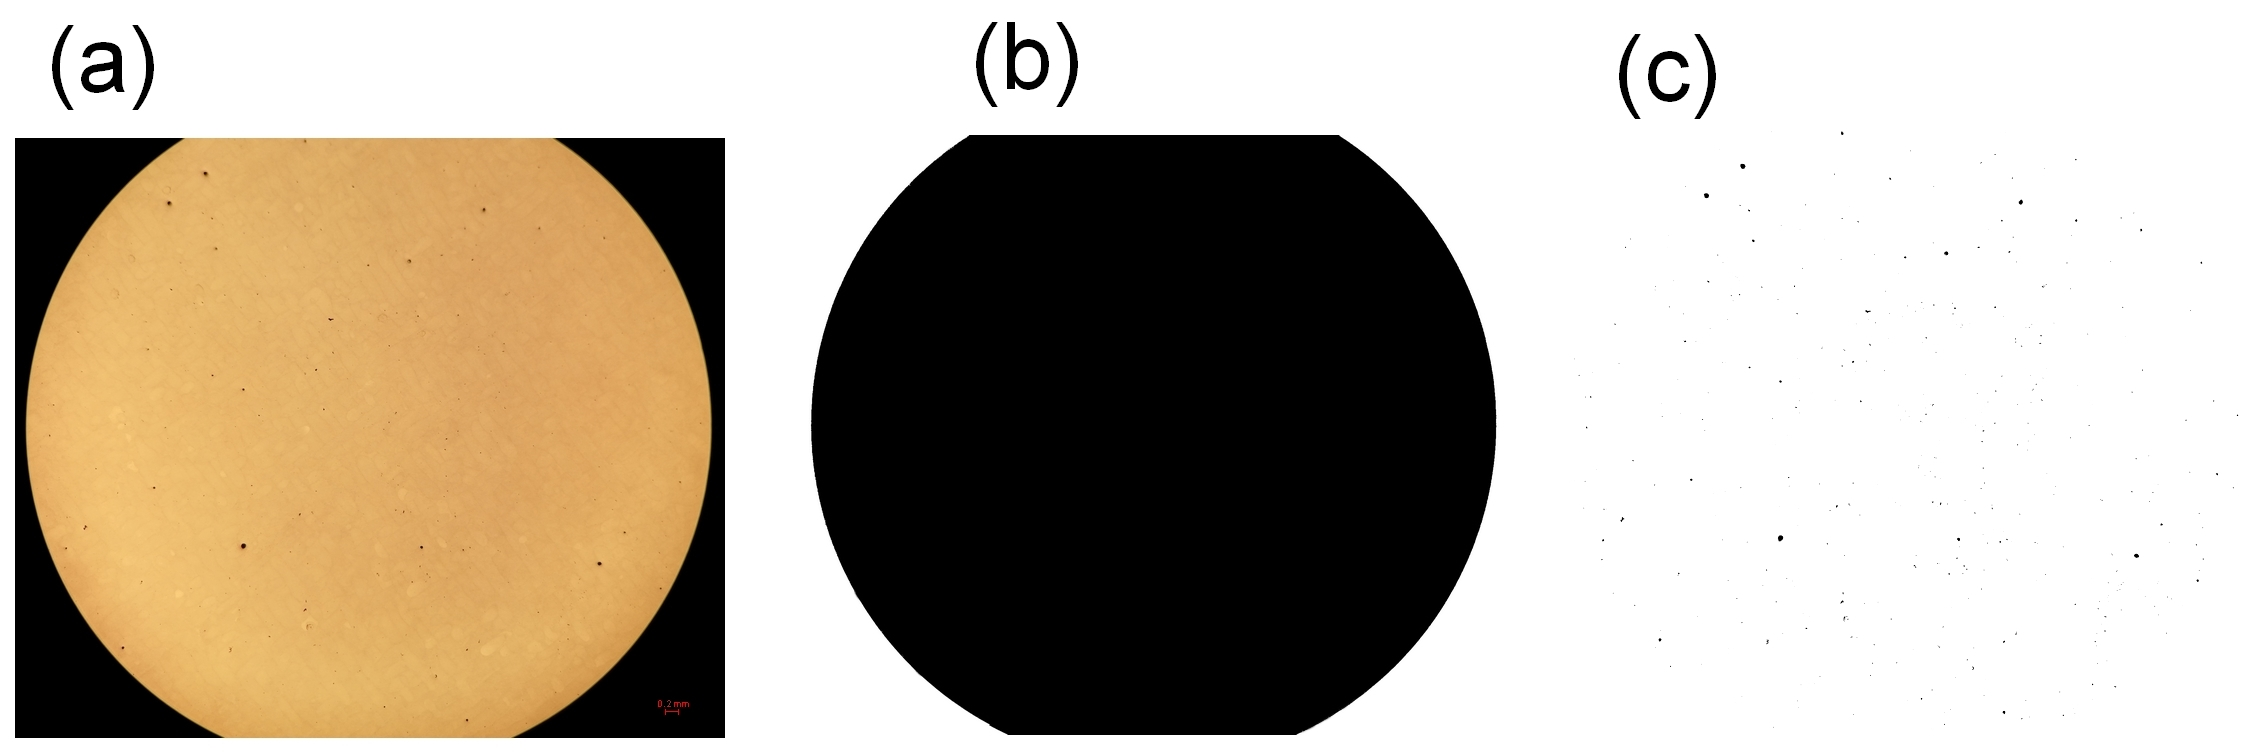
\includegraphics[scale=0.29]{Images/ImageJ-cub1}}
\decoRule
\caption[RODIA procedure for specimen X200-180319-cub 1: (a) Original picture of polished section (b) Whole surface isolation with \textit{ImageJ} (c) Porosities isolation with \textit{ImageJ}.]{RODIA procedure for specimen X200-180319-cub 1: (a) Original picture of polished section (b) Whole surface isolation with \textit{ImageJ} (c) Porosities isolation with \textit{ImageJ}.}
\label{fig:ImageJ}
\end{figure}

The images isolations in "foregrounds" and "backgrounds" were done trough manual thresholding based on pixel intensity quantifications.  %https://imagej.net/Thresholding#Global_thresholding
An optimal threshold was sought for porosities isolation so as to include only holes, and as many as possible. Particular attention was given to the photography in order to obtain the best contrast, focus and intensity homogeneity.

\subsection{Microscopy}

\subsubsection{Scanning electron microscopy}

\subsubsection{Optical microscopy}
Mesures Taille de bains

\subsection{Composition}

\subsection{Mechanical properties}

\subsubsection{Hardness test}

Vickers hardness measurements were made with a \textit{Wolpert Dia-Testor 2RC} tester. All analysed specimens were previously cut with a micro-cutting machine for the purpose of observing their bulk hardness. For each test, a pyramidal indenter (see figure \ref{fig:Vick}) was pressed on the samples surfaces with a load of 10 [kg] during 10 [sec]. The indentation durations were measured with a digital timer and the tests were stopped manually. The two diagonals lengths of the resulting indents were then evaluated using a ruler on the screen of the machine, which displays an image of the sample's surface captured by an embedded optical microscope.\\

\begin{figure}[th]
\centering
\centerline{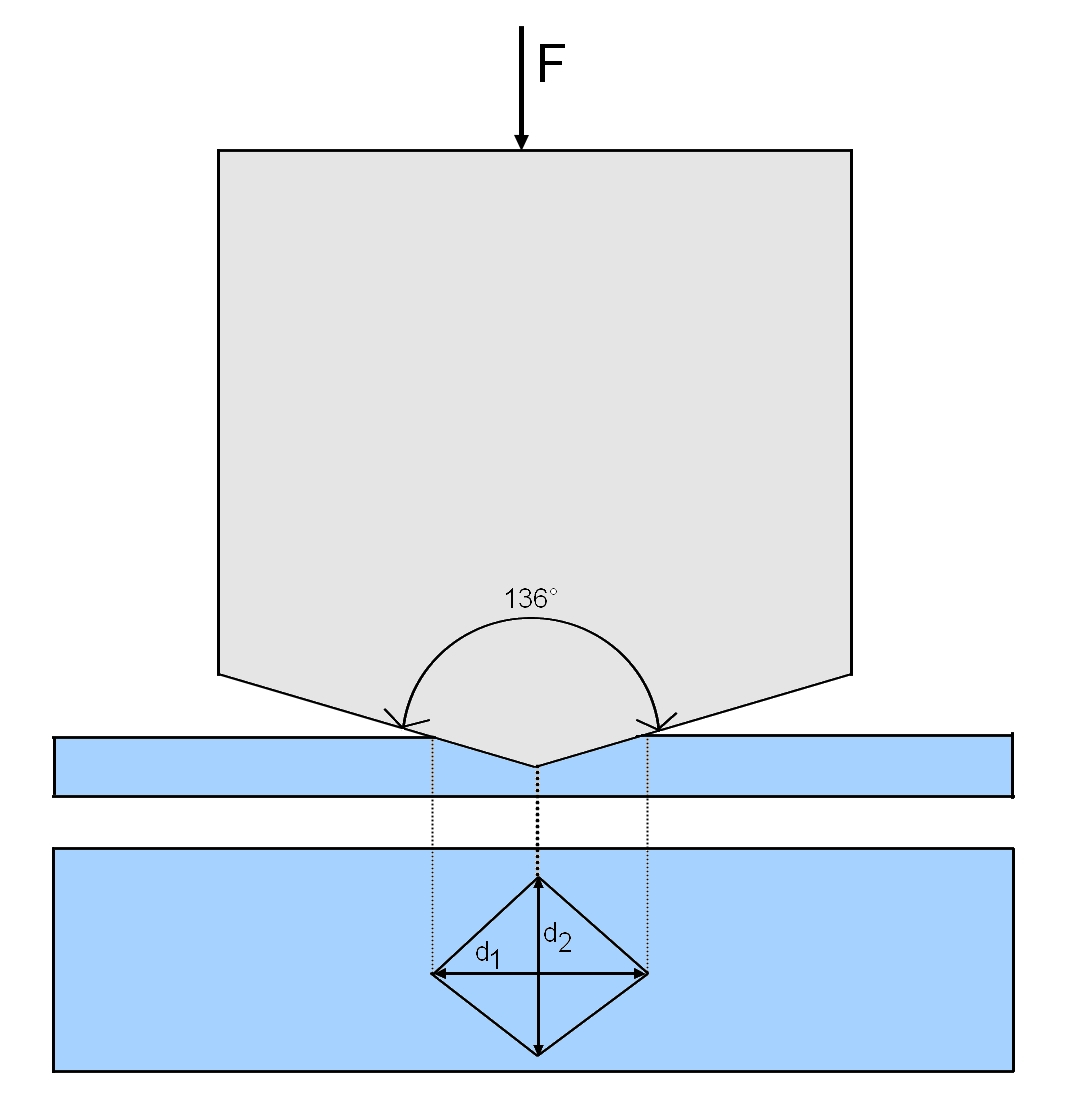
\includegraphics[scale=0.29]{Images/Vickers}}
\decoRule
\caption[Schematization of the Vickers hardness test]{Schematization of the Vickers hardness test}
\label{fig:Vick}
\end{figure}

Multiple tests were made for every samples and the mean diagonal length value was computed for each test. The corresponding Vickers harness values HV could then be found using a conversion table.\\

\subsubsection{Tensile test}

Machine?

%\subsubsection{Fatigue}
